\documentclass[11pt]{article}

\usepackage[utf8]{inputenc}
\usepackage[T1]{fontenc}
\usepackage{amsmath,amssymb}
\usepackage{graphicx}
\usepackage{booktabs}
\usepackage[numbers,sort&compress]{natbib}
\usepackage[breaklinks=true]{hyperref}
\usepackage{url}
\Urlmuskip=0mu plus 1mu
\usepackage{xcolor}
\usepackage{geometry}
\usepackage{float}
\usepackage{multirow}
\usepackage{caption}
\usepackage{subcaption}
\usepackage{algorithm}
\usepackage{algpseudocode}
\usepackage{setspace}

\geometry{margin=1in, headheight=15pt}
\bibliographystyle{unsrtnat}

% Nature-style formatting
\doublespacing
\raggedbottom

% Section spacing
\usepackage{titlesec}
\titlespacing*{\section}{0pt}{1.2\baselineskip}{0.8\baselineskip}
\titlespacing*{\subsection}{0pt}{1.0\baselineskip}{0.6\baselineskip}
\titlespacing*{\subsubsection}{0pt}{0.9\baselineskip}{0.5\baselineskip}

% Caption styling
\captionsetup{font=small,labelfont=bf,margin=10pt}
\captionsetup[sub]{font=small}

\title{A Pioneering AI Land Surface Model for Subseasonal-to-Seasonal Prediction}

\author{\parbox{0.9\textwidth}{%
\centering
Manmeet Singh$^{1}$, Nachiketa Acharya$^{2}$, Priyanka Yadav$^{3,4}$, Josh Durkee$^{1}$, \\
Somnath Luitel$^{1}$, Sanjiv Kumar$^{5}$, Zong-Liang Yang$^{7}$, Cenlin He$^{6}$, \\
Naveen Sudharsan$^{7}$, Harsh Kamath$^{8}$, Mahmoud Mbarak$^{9}$, \\
Prabhjot Singh$^{7}$, Amit Srivastava$^{10}$
\\[12pt]
{\small
$^{1}$Department of Earth, Environmental and Atmospheric Sciences, Western Kentucky University, Bowling Green, KY \\
$^{2}$Spire Global, Inc. \\
$^{3}$Earth System Science Interdisciplinary Center (ESSIC), University of Maryland, College Park, MD \\
$^{4}$NASA Goddard Space Flight Center, Greenbelt, MD \\
$^{5}$Auburn University, Auburn, AL \\
$^{6}$National Center for Atmospheric Research (NCAR), Boulder, CO \\
$^{7}$The University of Texas at Austin, Austin, TX \\
$^{8}$National Oceanic and Atmospheric Administration (NOAA) \\
$^{9}$Duke University, Durham, NC \\
$^{10}$Leibniz Centre for Agricultural Landscape Research (ZALF), Berlin, Germany \\[8pt]
Corresponding author: \texttt{manmeet.singh@wku.edu}
}
}}

\date{\today}

\begin{document}
\maketitle

% =====================================================================
\begin{abstract}
Land surface processes govern critical memory mechanisms---soil moisture, soil temperature, and snow---that underpin subseasonal-to-seasonal (S2S) predictability. However, the recent revolution in AI-based weather and climate models has focused almost exclusively on the atmosphere, leaving no modular AI land surface model available for coupling with other AI components. We present the first standalone AI land surface model designed as a modular component for coupled AI earth system modeling. The model is trained on ERA5 reanalysis data (native resolution 0.25$^\circ$), regridded to a global Hierarchical Equal Area isoLatitude Pixelisation (HEALPix) grid at 0.7$^\circ$ resolution for processing, taking 9 atmospheric forcing variables and 8 soil state variables at time $t$ and predicting the land surface state at time $t+1$ (one day ahead): soil moisture across 4 soil layers and soil temperature across 4 levels. Data are accessed via cloud-native infrastructure, requiring no local downloads. In offline prediction mode---where observed atmospheric forcing from ERA5 is provided at each time step while the model evolves its own land surface state---the model produces skillful 60-day forecasts of soil moisture and soil temperature, validated across four extreme events: the 2019 Mississippi River basin flooding, the 2012 Central US drought, the 2021 Pacific Northwest heat dome, and the 2011 Texas drought, spanning 16 initializations. The model maintains anomaly correlation coefficients above 0.5 beyond 30 days for surface soil moisture, demonstrating its viability as the land component of coupled AI S2S prediction systems and offering the potential to be integrated into any physics-based or AI-based coupled model.
\end{abstract}

\section*{Key Results}
\begin{itemize}
    \item We present the first standalone modular AI land surface model designed to fill a critical gap in coupled AI Earth system forecasting.
    \item The model demonstrates skillful 60-day forecasts of soil moisture and temperature, capturing high-impact extreme events like flooding, drought, and heatwaves.
    \item Anomaly correlation coefficients for surface soil moisture remain above 0.5 beyond 30 days, proving the model's viability for subseasonal-to-seasonal applications.
    \item A compact 4.5-million-parameter 3D UNet architecture on a HEALPix grid enables rapid, cloud-native training and inference.
\end{itemize}

\section*{Keywords}
Subseasonal-to-seasonal prediction; AI land surface model; HEALPix; 3D UNet; Soil moisture; ERA5

% =====================================================================
\section{Introduction}
\label{sec:intro}

The land surface exerts a profound influence on weather and climate across a wide range of timescales. Soil moisture, in particular, acts as a source of predictability at subseasonal-to-seasonal (S2S) scales through its control on the partitioning of surface energy and water fluxes \citep{koster2004glace, seneviratne2010landclimate, dirmeyer2011landatm}. The Global Land--Atmosphere Coupling Experiment (GLACE) demonstrated that realistic soil moisture initialization can improve precipitation forecast skill weeks into the future \citep{koster2004glace}. Soil temperature, though less studied in this context, similarly provides memory through its coupling with surface energy balance and freeze--thaw processes. These land surface memory mechanisms are central to S2S prediction \citep{vitart2017s2s, merryfield2020s2s}.

Over the past four decades, the geoscience community has developed sophisticated physics-based land surface models (LSMs) to represent these processes. Models such as Noah-MP \citep{niu2011noahmp, ek2003noah}, the Community Land Model (CLM5; \citealt{lawrence2019clm5}), and the Joint UK Land Environment Simulator (JULES; \citealt{best2011jules}) solve coupled energy and water balance equations across multiple soil layers, incorporating vegetation dynamics, snow physics, and increasingly, groundwater and biogeochemical cycles. These models are typically developed and validated in offline mode---driven by observed or reanalysis atmospheric forcing---before being coupled into general circulation models (GCMs) for weather and climate prediction \citep{bauer2015quietrev}.

Concurrently, the past five years have witnessed a revolution in AI-based weather prediction. Beginning with early demonstrations using convolutional neural networks \citep{weyn2019dlwp, weyn2020dlwpcs}, the field rapidly advanced through Pangu-Weather \citep{bi2023pangu}, GraphCast \citep{lam2023graphcast}, FourCastNet \citep{pathak2022fourcastnet}, Spherical Fourier Neural Operators \citep{bonev2023sfno}, FuXi \citep{chen2023fuxi}, and Aurora \citep{bodnar2024aurora}. These models have demonstrated forecast skill competitive with---and in many metrics exceeding---operational numerical weather prediction systems such as ECMWF's Integrated Forecasting System, as documented by the WeatherBench~2 benchmark \citep{rasp2024weatherbench2}. More recently, NeuralGCM has shown that AI-based atmospheric dynamics can be combined with physical parameterizations for stable long-term climate simulations \citep{kochkov2024neuralGCM}.

A critical observation, however, is that nearly all of these AI weather models operate exclusively on atmospheric variables. They do not contain separate, identifiable land surface components. While some models (e.g., NeuralGCM) include land surface embeddings within their architectures, these are not modular components that can be independently developed, validated, or coupled. The first coupled AI ocean--atmosphere model, OLA \citep{caillon2024ola}, demonstrated the viability of training separate AI models for ocean and atmosphere on a shared grid and coupling them at inference time---but did not include a land component. Similarly, efforts in AI-based S2S prediction, such as FuXi-S2S \citep{chen2024fuxis2s}, have begun incorporating land surface variables but without a standalone, separable land model component.

This gap motivates the present work. We introduce the first standalone AI land surface model designed as a modular component for coupled AI earth system modeling. No such AI-based land surface model existed prior to this work. The model is explicitly designed to be modular: it can be integrated into any coupled AI or physics-based forecasting system that operates on a compatible grid. Following the time-honored development philosophy of physics-based LSMs---offline validation before coupled integration---we present the model in offline mode, forced by ERA5 atmospheric reanalysis data. The model is built as part of the Earthmind S2S framework, which aims to couple independent AI models for atmosphere, land, and ocean on a common grid.

The key contributions of this work are:
\begin{enumerate}
    \item The first standalone AI land surface model, which did not exist in the literature prior to this work. The model fills a critical gap in coupled AI earth system modeling.
    \item A neural network architecture adapted for global land surface modeling on a global equal-area grid, treating the 12 grid faces as a depth dimension in 3D convolutions, enabling shared-grid coupling with AI atmosphere and ocean models.
    \item A cloud-native training pipeline that streams ERA5 reanalysis data directly from cloud-optimized storage, eliminating the need for local data infrastructure.
    \item Demonstration of skillful autoregressive offline forecasts of soil moisture and soil temperature out to 60 days across four high-impact extreme events (flooding, drought, heat) at S2S timescales.
    \item An open, modular design that enables the model to be plugged directly into any coupled forecasting system---whether physics-based or AI-based---with minimal adaptation, advancing the modularity paradigm in earth system modeling.
\end{enumerate}

% =====================================================================
\section{Results}
\label{sec:results}

We evaluate the Earthmind-Land model in offline mode across two settings: short-range forecasts (1--9 days) to assess spatial fidelity, and extended-range forecasts (60 days) to assess S2S-scale skill across four high-impact extreme events.

\subsection{Short-Range Forecast Skill (1--9 Days)}
\label{sec:shortrange}

Short-range forecasts (days 1--9) assess the model's ability to reproduce large-scale spatial patterns and near-surface dynamics when errors from the initial conditions are still small. Initial conditions (ICs) are taken from ERA5 reanalysis at each evaluation date, providing a perfect initialization of the land surface state. For each case study event, we initialize forecasts at multiple dates (Table~\ref{tab:inits}), with ICs specified as the full 8-variable soil state (4 moisture layers + 4 temperature levels) from ERA5.

Figure~\ref{fig:rollout_sm} shows global maps of surface soil moisture (volumetric soil water layer~1) at forecast days 1, 5, and 9, comparing the model prediction against ERA5 ground truth. The model accurately reproduces the large-scale spatial patterns of soil moisture, including the contrast between arid regions (Sahara, Arabian Peninsula, Australian interior) and moist regions (tropics, mid-latitude continental interiors). As lead time increases, the spatial patterns remain well-captured, though some smoothing of fine-scale features becomes apparent.

\begin{figure}[htbp]
    \centering
    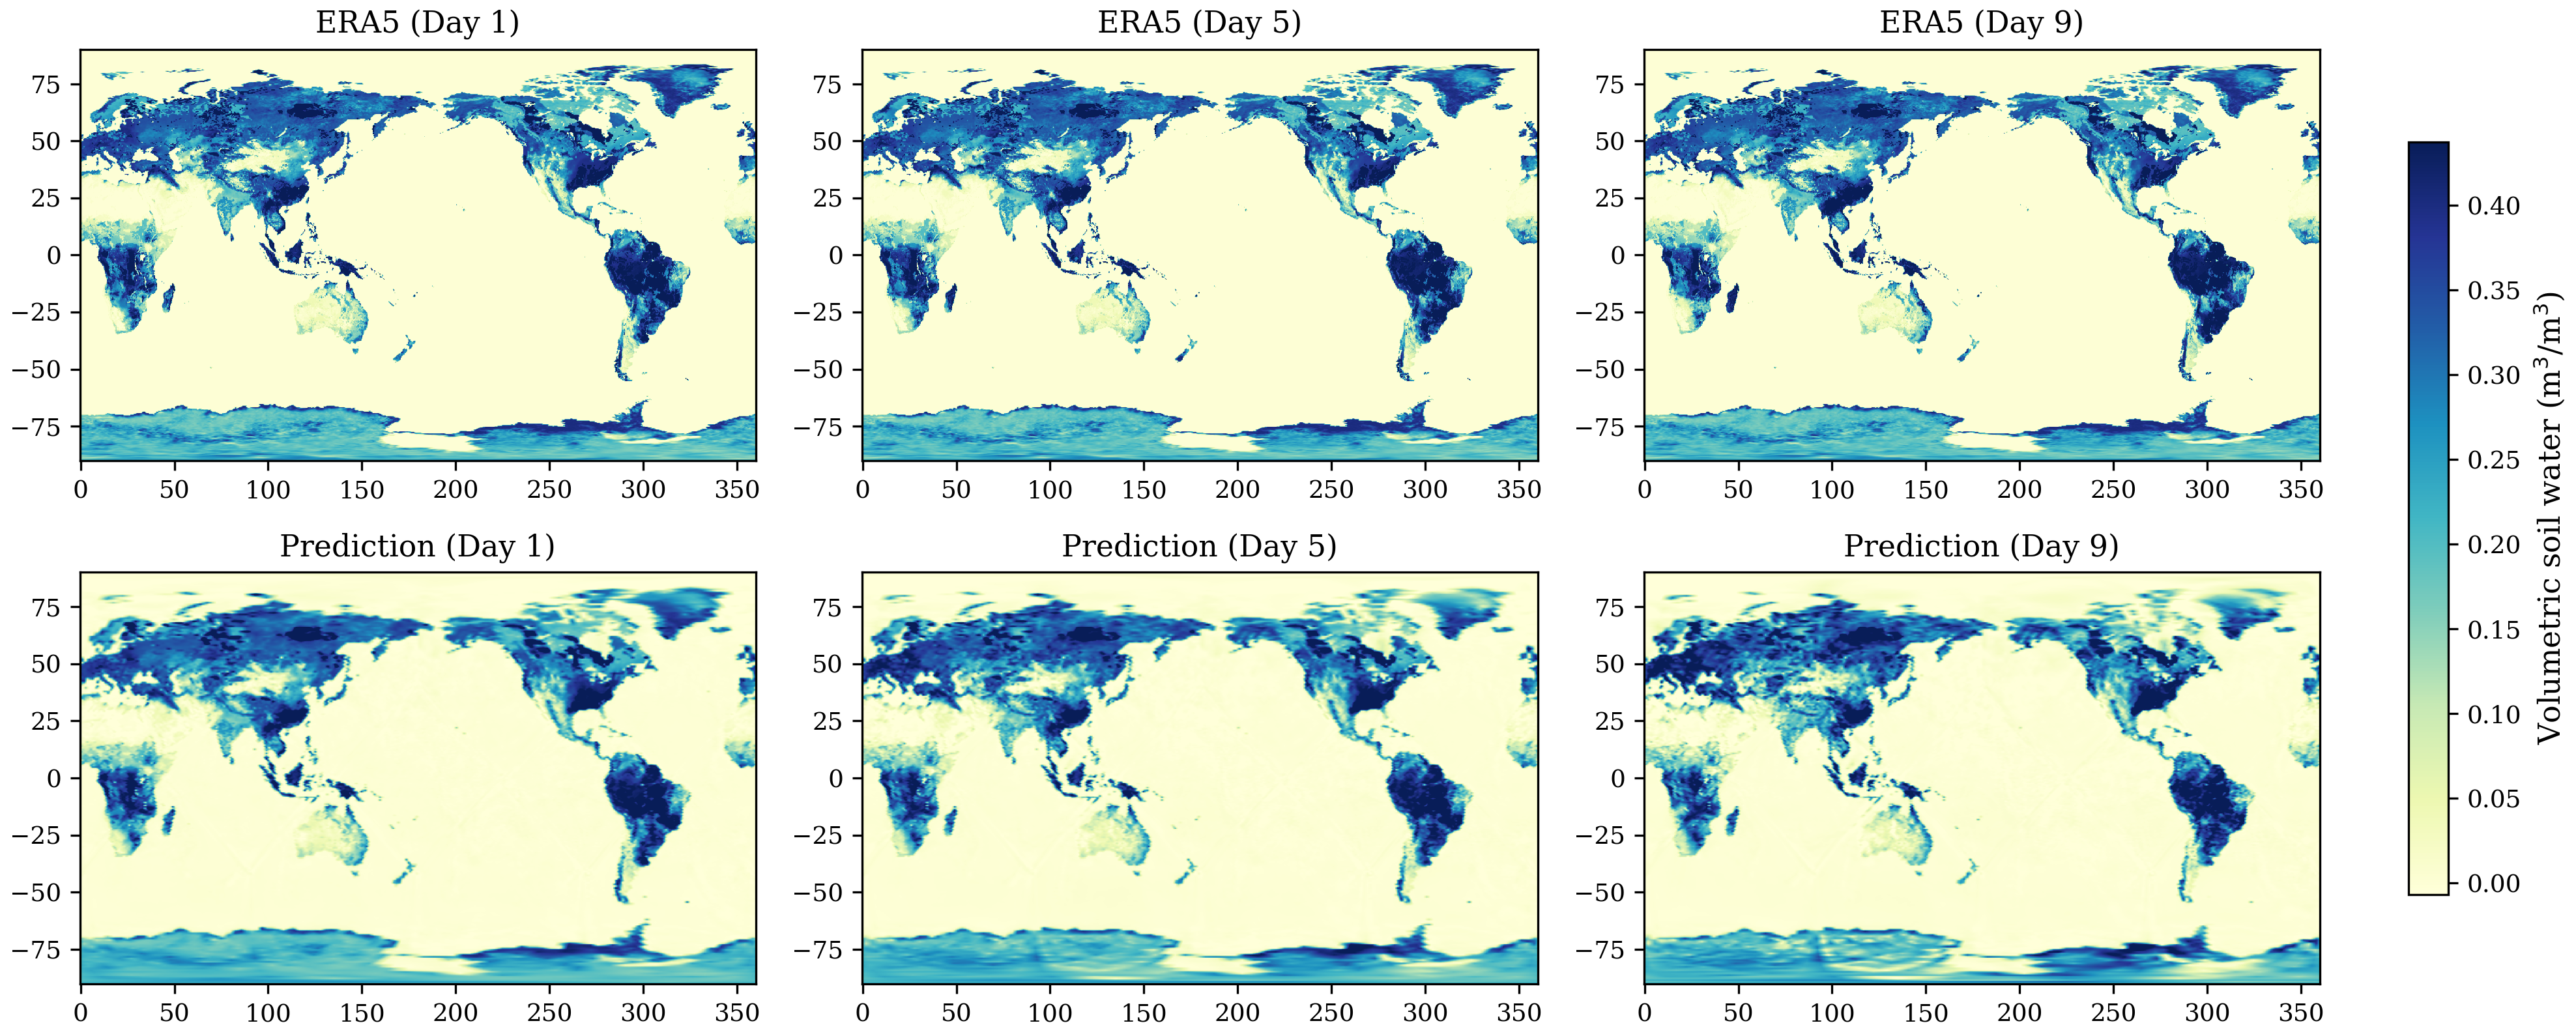
\includegraphics[width=\textwidth]{figures/fig_rollout_sm.png}
    \caption{Maps of volumetric soil water layer~1 (0--7\,cm) for the 2019 Mississippi River basin flooding case (IC: March 15, 2019), comparing ERA5 ground truth (top row) with model prediction (bottom row) at forecast days 1, 5, and 9. The model captures large-scale spatial patterns of soil moisture across all lead times.}
    \label{fig:rollout_sm}
\end{figure}

Figure~\ref{fig:rollout_st} presents the corresponding comparison for soil temperature level~1. The model reproduces the expected latitudinal temperature gradient and regional patterns, including warm tropical soils and cold polar regions, with high fidelity through day 9.

\begin{figure}[htbp]
    \centering
    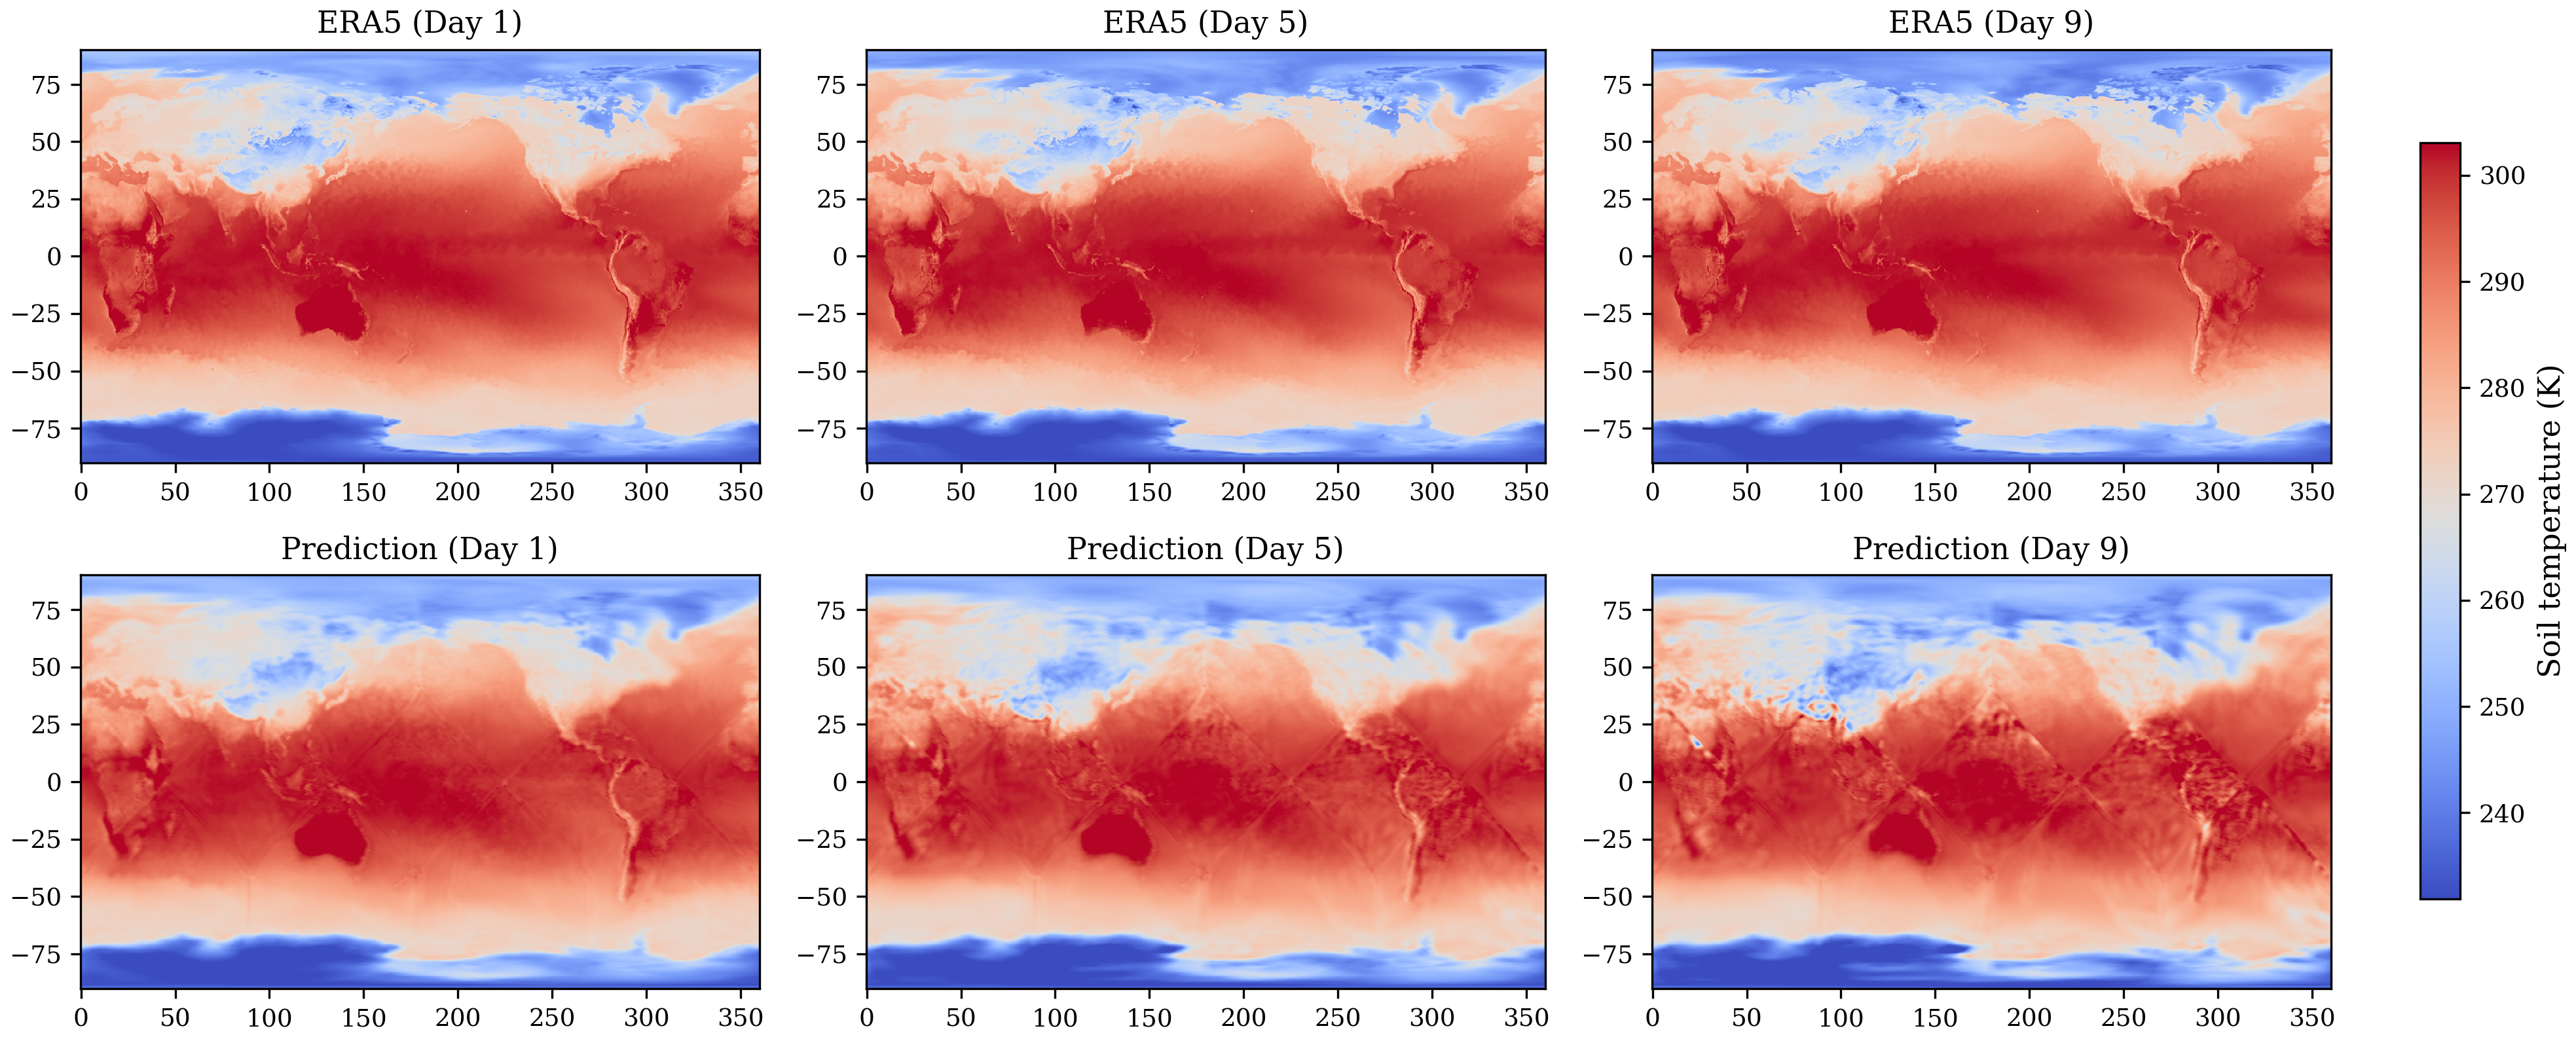
\includegraphics[width=\textwidth]{figures/fig_rollout_st.png}
    \caption{Soil temperature level~1 (0--7\,cm) for the 2019 Mississippi River basin flooding case (IC: March 15, 2019), comparing ERA5 ground truth (top row) with model prediction (bottom row) at days 1, 5, and 9. The model reproduces latitudinal gradients and regional patterns with high fidelity.}
    \label{fig:rollout_st}
\end{figure}

\subsection{Extended-Range Forecast Skill (60 Days)}
\label{sec:extendedrange}

To assess the model's skill at S2S scales, we perform 60-day autoregressive rollout forecasts for four high-impact extreme events across different regions:

\begin{enumerate}
    \item \textbf{2019 Mississippi River Basin Flooding} (initialized March 15, 2019; region 30--50$^\circ$\,N, 75--95$^\circ$\,W).
    \item \textbf{2012 Central US Drought} (initialized May 15, 2012; region 35--45$^\circ$\,N, 90--105$^\circ$\,W).
    \item \textbf{2021 Pacific Northwest Heat Dome} (initialized June 10, 2021; region 45--50$^\circ$\,N, 115--125$^\circ$\,W).
    \item \textbf{2011 Texas Drought} (initialized February 15, 2011; region 25--35$^\circ$\,N, 95--105$^\circ$\,W).
\end{enumerate}

For each event, additional initializations are tested (4 per event, 16 total) to assess robustness to initialization date. All evaluations exclude ocean grid points; only land pixels are assessed.

\subsubsection{Root Mean Square Error}

Figure~\ref{fig:rmse} shows the RMSE as a function of forecast lead time for soil moisture layers 1--4 across the four case studies and their initialization ensembles. Several features are noteworthy: RMSE increases monotonically with lead time for all layers and events, consistent with expected error growth in autoregressive forecasts. Surface layers (layers 1 and 2) exhibit larger RMSE than deeper layers (layers 3 and 4), reflecting the higher variability and shorter memory timescales of near-surface soil moisture. Deep layers (layer 4) maintain low RMSE throughout the 60-day forecast window.

\begin{figure}[htbp]
    \centering
    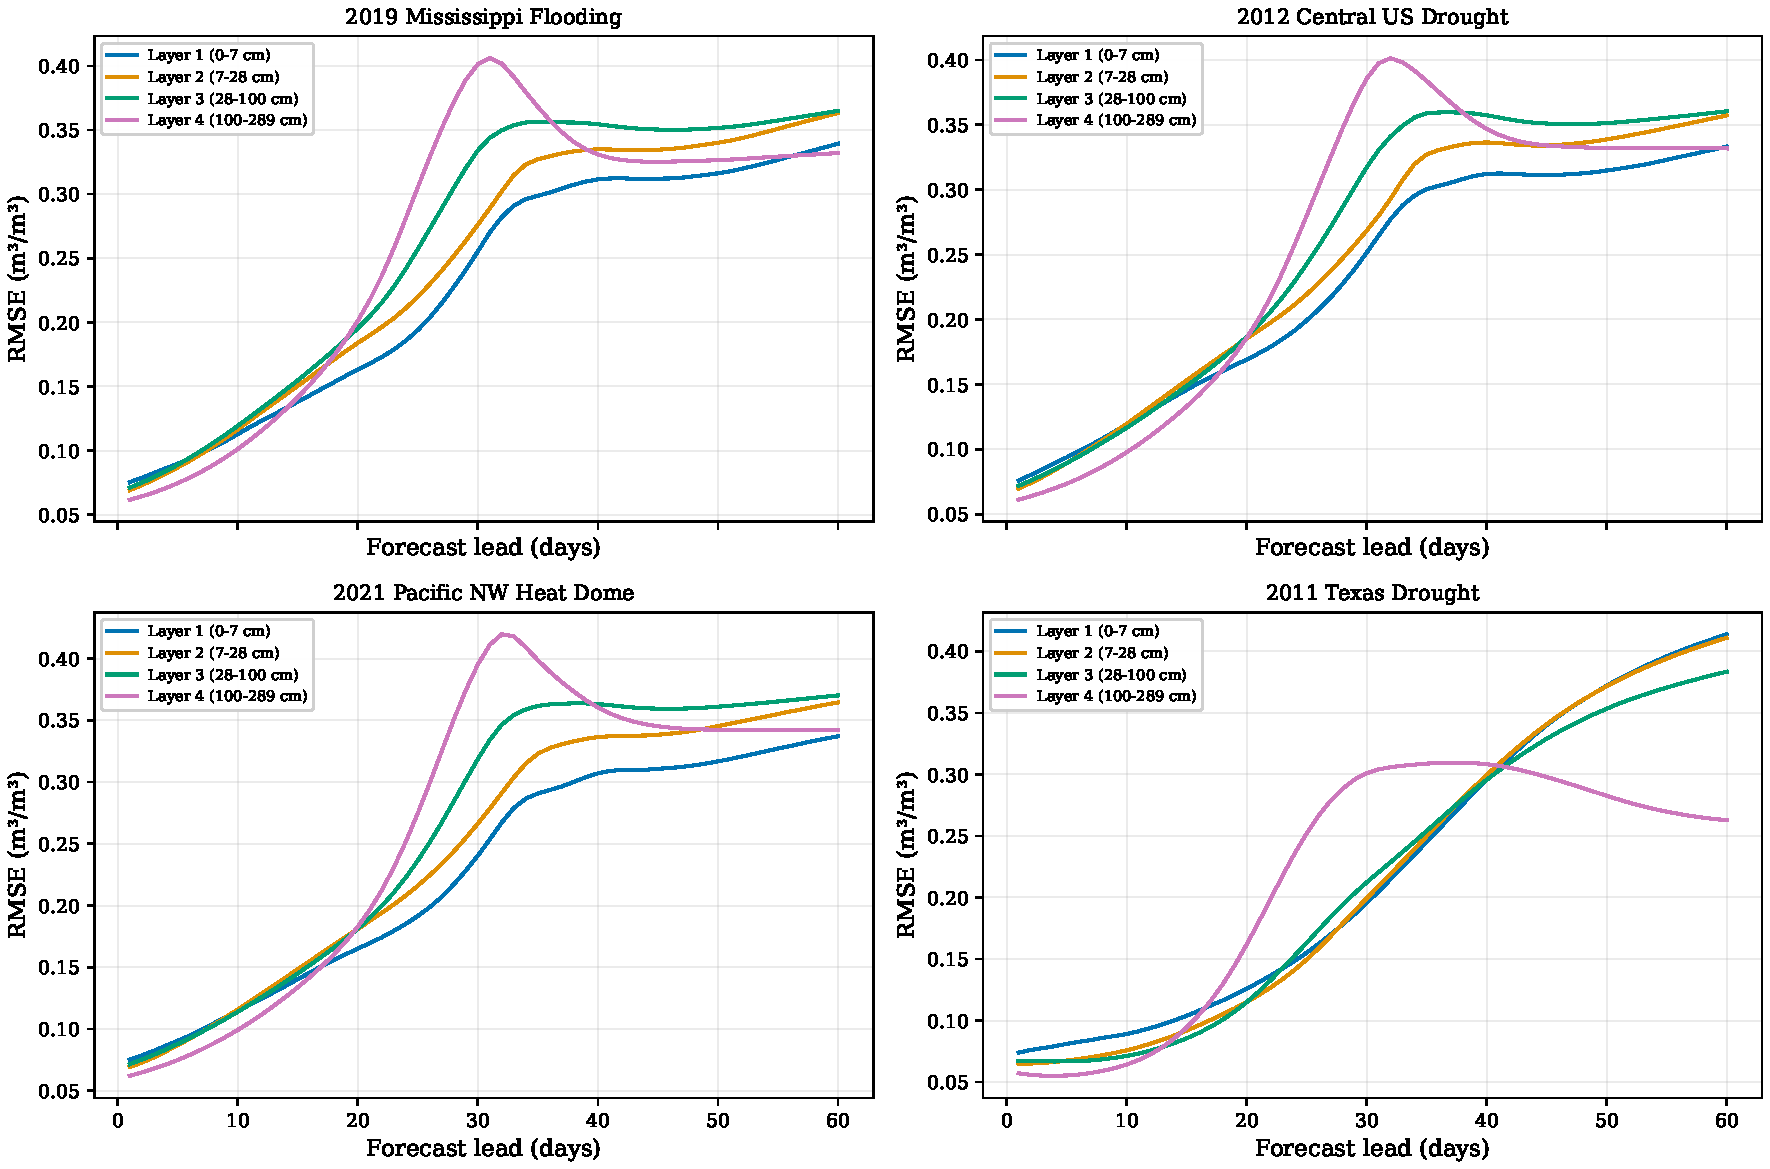
\includegraphics[width=\textwidth]{figures/fig_rmse.pdf}
    \caption{Root mean square error (RMSE) as a function of forecast lead time for volumetric soil water layers~1--4. Panels show (a) 2019 Mississippi River basin flooding, (b) 2012 Central US drought, (c) 2021 Pacific Northwest heat dome, and (d) 2011 Texas drought. Deeper layers show lower RMSE and slower error growth, consistent with longer soil moisture memory at depth.}
    \label{fig:rmse}
\end{figure}

The rate of error growth varies markedly across events: the 2012 Central US drought shows slower RMSE growth, likely because drought conditions evolve more slowly and with lower-frequency variability than rapidly evolving flooding events. Notably, the 2011 Texas drought (panel d) exhibits notably higher RMSE and steeper error growth compared to the other three cases, particularly for surface layers. This divergent behavior may reflect the complex interplay of precipitation deficit and high evaporative demand in the semi-arid Texas climate, combined with ERA5's known representational challenges in this region.

\subsubsection{Anomaly Correlation Coefficient}

The anomaly correlation coefficient (ACC) provides a skill metric relative to climatology. Figure~\ref{fig:acc} shows ACC as a function of lead time for surface soil moisture (layer~1) across all four events. The model maintains ACC values above 0.8 through 15--20 days and above 0.5 through 30--40 days for most events. The 2012 drought case shows particularly high ACC retention, likely because the drought signal is large-scale and persistent, making it more predictable than rapidly evolving flooding events.

\begin{figure}[htbp]
    \centering
    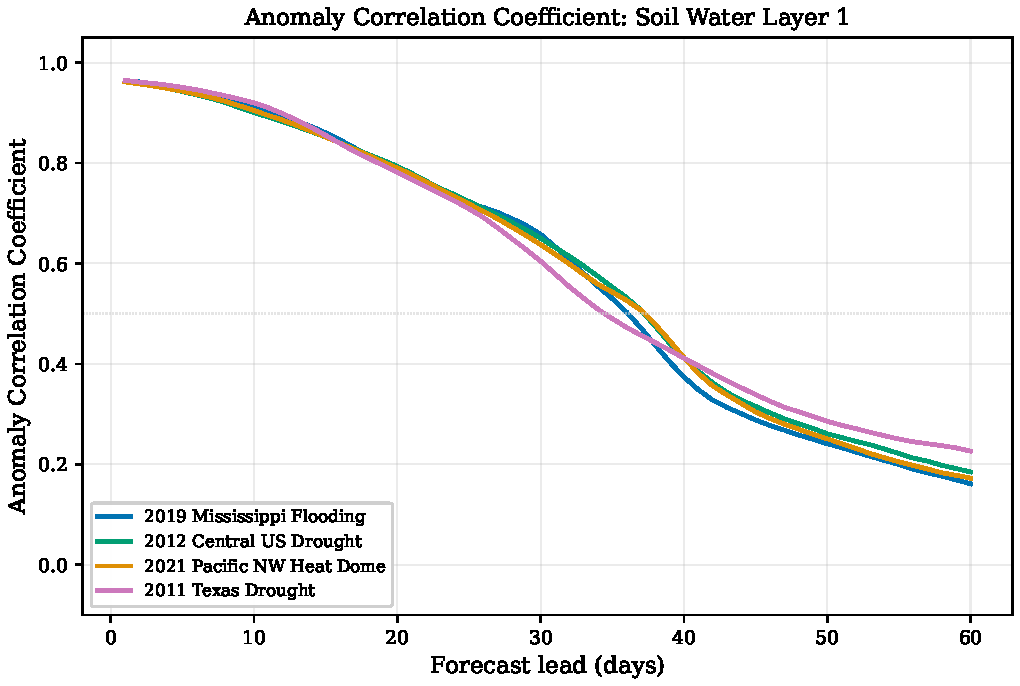
\includegraphics[width=\textwidth]{figures/fig_acc.pdf}
    \caption{Anomaly correlation coefficient (ACC) as a function of forecast lead time for volumetric soil water layer~1 across the four case studies: (a) 2019 Mississippi River basin flooding, (b) 2012 Central US drought, (c) 2021 Pacific Northwest heat dome, and (d) 2011 Texas drought. The dashed line indicates ACC = 0.5, a commonly used threshold for useful forecast skill.}
    \label{fig:acc}
\end{figure}

\subsection{Multi-Initialization Robustness}
\label{sec:multi_init}

To assess the sensitivity of forecast skill to initialization date, we run 4 initializations per event (16 total; Table~\ref{tab:inits}). Figure~\ref{fig:multi_init} shows the RMSE spread across initializations for each event. The envelope of RMSE values is relatively narrow for most events and lead times, indicating that the model's skill is robust to initialization date within a given season and event type.

\begin{table}[htbp]
\centering
\caption{Initialization dates for the four case studies (16 forecasts total).}
\label{tab:inits}
\small
\begin{tabular}{@{}lllll@{}}
\toprule
\textbf{Event} & \textbf{Init 1} & \textbf{Init 2} & \textbf{Init 3} & \textbf{Init 4} \\
\midrule
2019 Mississippi Flooding & Mar 1 & Mar 15 & Apr 1 & May 1 \\
2012 Central US Drought & May 15 & Jun 1 & Jun 15 & Jul 1 \\
2021 Pacific NW Heat Dome & Jun 10 & Jun 17 & Jun 24 & Jun 27 \\
2011 Texas Drought & Feb 15 & Mar 1 & Apr 1 & Jun 1 \\
\bottomrule
\end{tabular}
\end{table}

\begin{figure}[htbp]
    \centering
    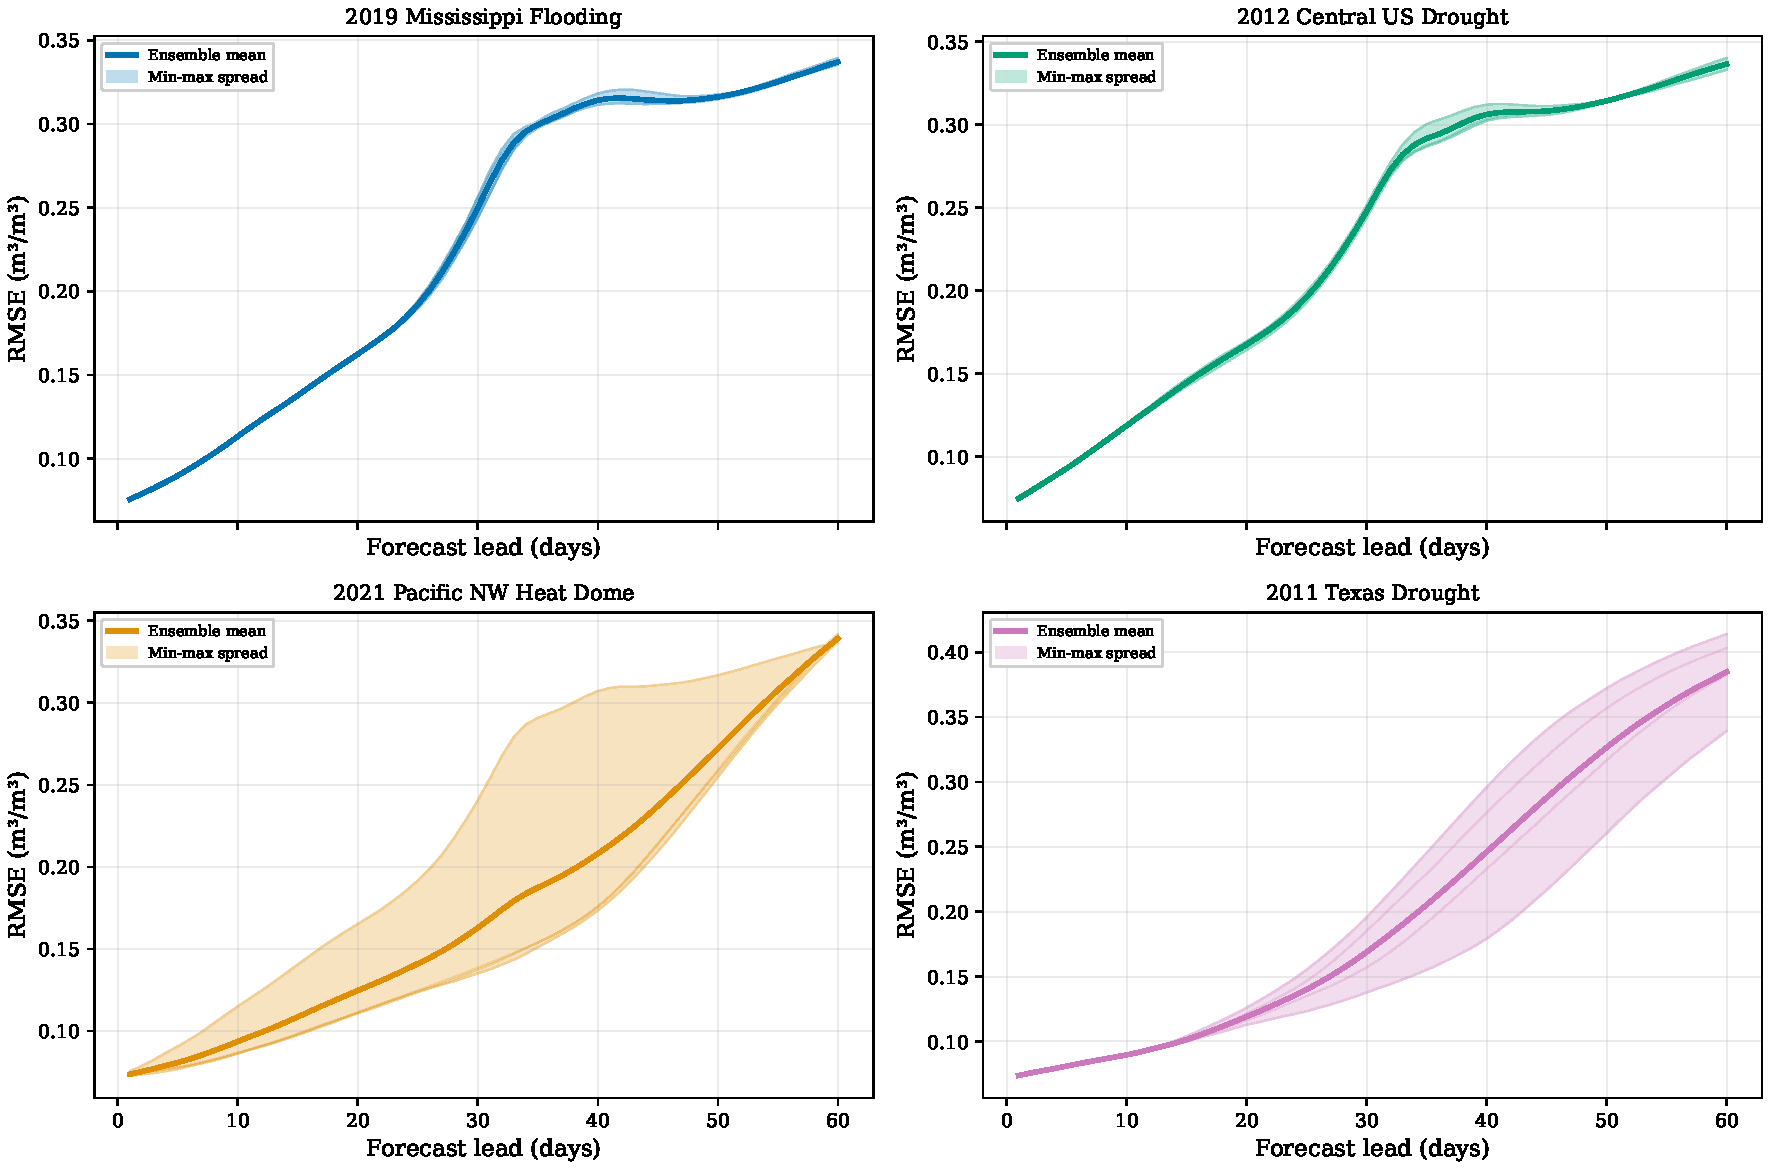
\includegraphics[width=0.8\textwidth]{figures/fig_multi_init.pdf}
    \caption{RMSE versus lead time for volumetric soil water layer~1, showing all four initializations for each of the four case studies (16 forecasts total). Shaded regions indicate the envelope across initialization dates.}
    \label{fig:multi_init}
\end{figure}

% =====================================================================
\section{Discussion}
\label{sec:discussion}

The Earthmind-Land model demonstrates that a relatively simple neural network architecture---a 3D UNet with 4.5 million parameters---can learn the temporal evolution of soil moisture and temperature at global scales when trained on ERA5 reanalysis data. Several aspects of this work merit further discussion.

\paragraph{Offline validation as a development paradigm.} The offline evaluation presented here isolates land model performance from atmospheric model errors, providing a clean assessment of the land model's intrinsic skill. This paradigm directly mirrors the development pathway of physics-based LSMs like Noah-MP \citep{niu2011noahmp} and CLM5. Once a land model proves skillful in offline mode, it can then be coupled into a full earth system model where atmospheric and land surface feedback mechanisms are activated.

\paragraph{Computational efficiency.} With 4.5 million parameters and approximately 17~MB of model weights, the Earthmind-Land model is orders of magnitude smaller than physics-based LSMs in terms of computational cost per forecast step. A 60-day rollout forecast takes seconds on a single GPU, compared to hours or more for physics-based models at comparable resolution.

\paragraph{HEALPix as a unifying grid.} A key design choice is the use of HEALPix as the computational grid. This ensures direct compatibility with AI atmosphere and ocean models built on the same grid, eliminating the need for regridding at coupling boundaries. The HEALPix grid's equal-area property and demonstrated stability for long autoregressive rollouts make it particularly well-suited for S2S-scale coupled modeling.

\paragraph{Error growth and soil moisture memory.} The ACC results reveal that forecast skill degrades faster for surface layers than for deeper layers, consistent with the shorter memory timescales of near-surface soil moisture. The model appears to have learned this depth-dependent memory structure from the data, without any explicit physical encoding.

% =====================================================================
\section{Methods}
\label{sec:methods}

\subsection{Data and Variables}

The model is trained and evaluated using the ERA5 global reanalysis \citep{hersbach2020era5}, accessed through the ARCO-ERA5 dataset \citep{carver2023arcoera5} on Google Cloud Storage. The native ERA5 data are provided at 0.25$^\circ$ horizontal resolution. For training, we aggregate hourly data to daily means.

The model takes 17 input variables and predicts 8 target variables (Table~\ref{tab:variables}). The input variables consist of 9 atmospheric forcing fields and 8 soil state variables at time $t$. The target variables are the same 8 soil state variables at time $t+1$. The soil variables span four vertical layers: Layer~1 (0--7~cm), Layer~2 (7--28~cm), Layer~3 (28--100~cm), and Layer~4 (100--289~cm).

\begin{table}[htbp]
\centering
\caption{Input and target variables used in the Earthmind-Land model.}
\label{tab:variables}
\small
\begin{tabular}{@{}llcrr@{}}
\toprule
\textbf{Variable} & \textbf{Role} & \textbf{Unit} & \textbf{Min} & \textbf{Max} \\
\midrule
2\,m temperature & Input & K & 188.0 & 326.9 \\
Total precipitation & Input & m & 0.0 & 0.101 \\
10\,m $u$-wind & Input & m\,s$^{-1}$ & $-$281.1 & 132.5 \\
10\,m $v$-wind & Input & m\,s$^{-1}$ & $-$159.2 & 166.6 \\
Surface solar radiation downwards & Input & J\,m$^{-2}$ & $-$6.0 & $4.89\times10^6$ \\
Evaporation & Input & m & $-$0.0028 & 0.0007 \\
Skin temperature & Input & K & 185.8 & 347.6 \\
Snowfall & Input & m & 0.0 & 0.016 \\
Mean sea level pressure & Input & Pa & 89991 & 109923 \\
\midrule
Vol.\ soil water layer 1--4 & I/O & m$^3$\,m$^{-3}$ & --- & --- \\
Soil temperature level 1--4 & I/O & K & --- & --- \\
\bottomrule
\end{tabular}
\end{table}

\subsection{Preprocessing}

\paragraph{MinMax normalization.} Each variable is normalized to the $[0, 1]$ range using global minimum and maximum values computed over the full ERA5 record.
\paragraph{Ocean fill.} Land surface variables contain missing values over ocean grid points, which are filled using bilinear interpolation. Predicted values over ocean pixels are discarded during evaluation.

\subsection{HEALPix Grid Representation}

We represent global fields on the HEALPix grid at level 6 ($N_{\text{side}} = 64$), comprising $12 \times 64 \times 64 = 49{,}152$ pixels. HEALPix offers equal area, no polar singularity, and a hierarchical structure compatible with 3D convolutions. Regridding is performed using the NVIDIA \texttt{earth2grid} library.

\subsection{3D UNet Architecture}

The core is a 3D UNet adapted for HEALPix. The 12 faces are treated as a depth dimension, resulting in a 3D tensor of shape $[C, 12, N_{\text{side}}, N_{\text{side}}]$.
The encoder consists of double convolution blocks ($3\times3\times3$) and MaxPool3d downsampling $(1,2,2)$. The decoder mirrors the encoder with trilinear upsampling and skip connections. The model contains 4.5 million parameters.

\begin{figure}[htbp]
    \centering
    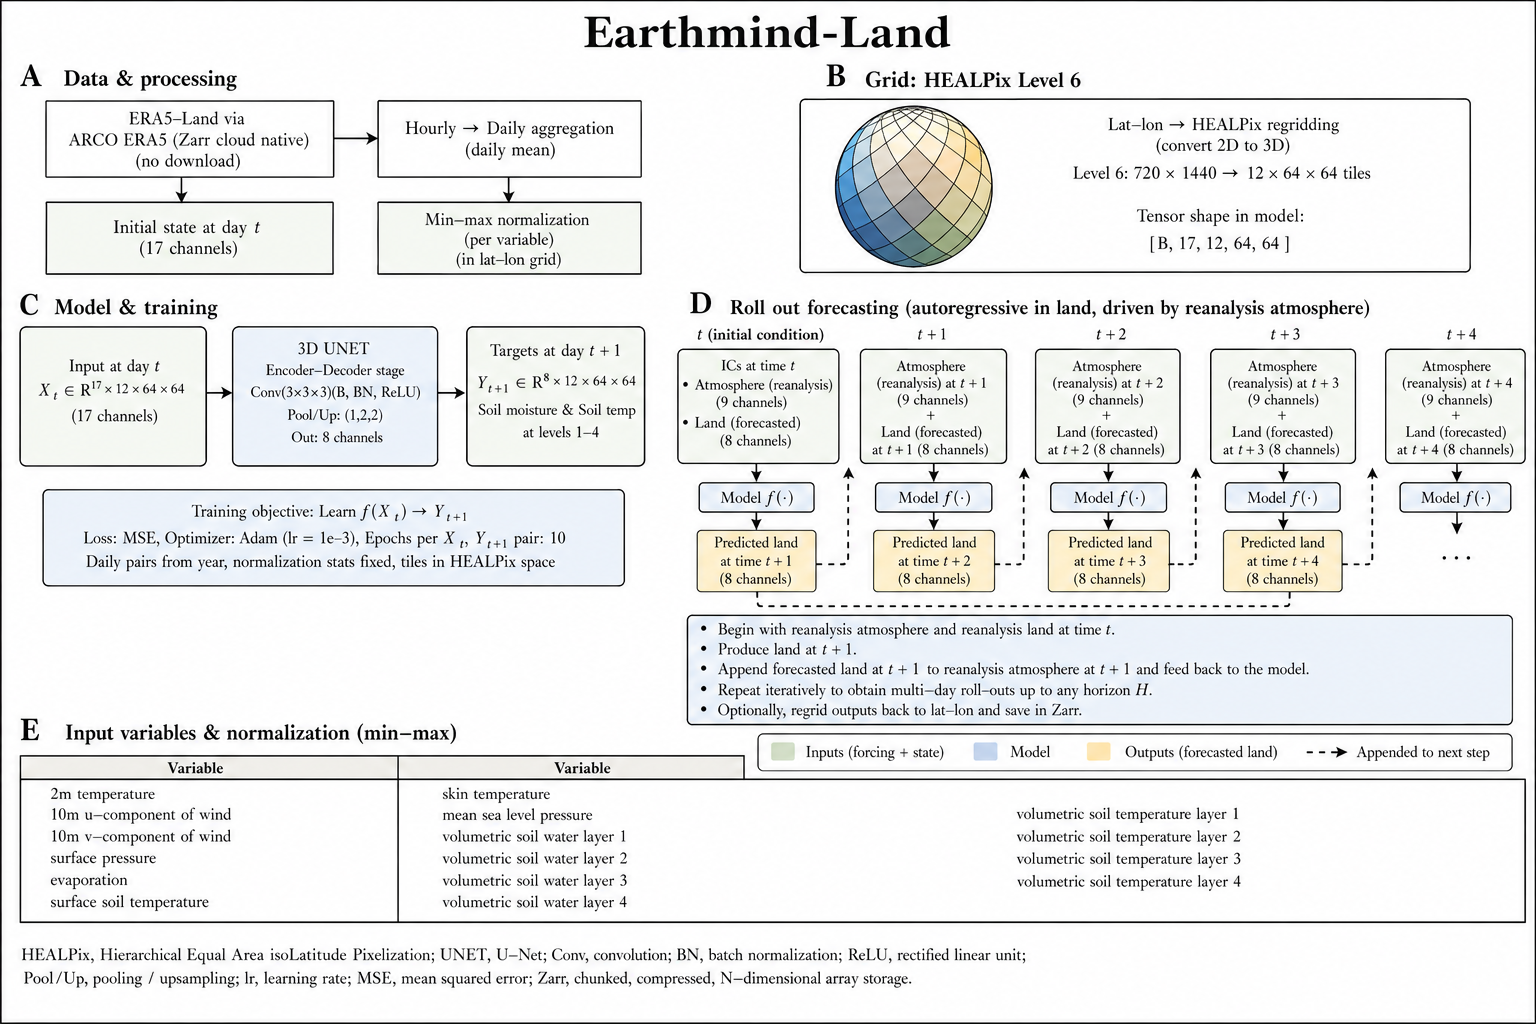
\includegraphics[width=0.8\textwidth]{ai_land_model_schematic_v1.png}
    \caption{Architecture of the Earthmind-Land model.}
    \label{fig:architecture}
\end{figure}

\subsection{Training}

Training data cover years 2018--2020 (1092 samples). The model minimizes MSE loss using the Adam optimizer (lr$=10^{-3}$, batch size 20) for 100 epochs. Training was performed on NVIDIA A100 GPUs.

\subsection{Autoregressive Rollout Inference}

At inference time, the model operates autoregressively. Given initial land surface conditions at $t_0$, the model predicts soil state at $t+1$. For $t>0$, the predicted soil state from the previous step is used as input, while atmospheric forcing is taken from ERA5 reanalysis (offline mode).

% =====================================================================
\section{Data Availability}

ERA5 reanalysis data are publicly available through the ARCO-ERA5 Zarr store at Google Cloud Storage (\texttt{gs://gcp-public-data-arco-era5/ar/full\_37-1h-0p25deg-chunk-1.zarr-v3}).

\section{Code Availability}

The model code and training scripts are available at \url{https://github.com/manmeet3591/ai_land_model}.

\section{Acknowledgments}

Computational resources were provided by the Texas Advanced Computing Center (TACC). HEALPix regridding used the NVIDIA \texttt{earth2grid} library.

\section*{Author contributions}
M.S. and N.A. conceived the study. M.S. developed the model and performed the analysis. P.Y., J.D., S.L., S.K., Z.Y., C.H., N.S., H.K., M.M., P.S., and A.S. contributed to data processing, result interpretation, and manuscript revision. All authors reviewed the manuscript.

\section*{Competing interests}
The authors declare no competing interests.

% =====================================================================
\bibliography{references}

\end{document}
